%!TEX root = ../StatisticalCorrelations.tex

\graphicspath{{Body/Figures/EvW/}}

\section{Monte Carlo}


In order to determine correlation coefficients between the various analyses, a Monte Carlo simulation was developed. This Monte Carlo generates pseudo-data according to the different analysis types, fills histograms defined by the parameters in \tabref{tab:analyzerParameters}, and then fits them accordingly. Pseudo-data was generated using \ROOT's \texttt{TF2->GetRandom2()} method. The 2D function used to generate the data is given by a five parameter function with energy dependence on the number, asymmetry, and phase terms,
\begin{align}
	N(t, E) = N_{0}(E) \cdot e^{-t/\tau_{\mu}} \cdot (1 + A(E) \cos{(\omega_{a}t + \phi(E))}),
\label{eq:2dfunc}
\end{align}
with the time-dilated muon lifetime \taumu equal to \ns{64440} and \gmtwo frequency \wa set as
\begin{align}
	\omega_{a} = 2\pi \cdot 0.2291 \text{MHz} \cdot (1 + R \times 10^{-6}),
\end{align}
where \R was set to 0. 


The energy dependent terms in \equref{eq:2dfunc} were determined from energy-binned fits to the data provided by D. Sweigart for ReconEast and M. Sorbara for ReconWest, for each of the four datasets in \Rone. 


- mention low and high energy thresholds, bin width and number of points, interpolation, 




\begin{figure}[]
\centering
    \begin{subfigure}[t]{0.45\textwidth}
        \centering
        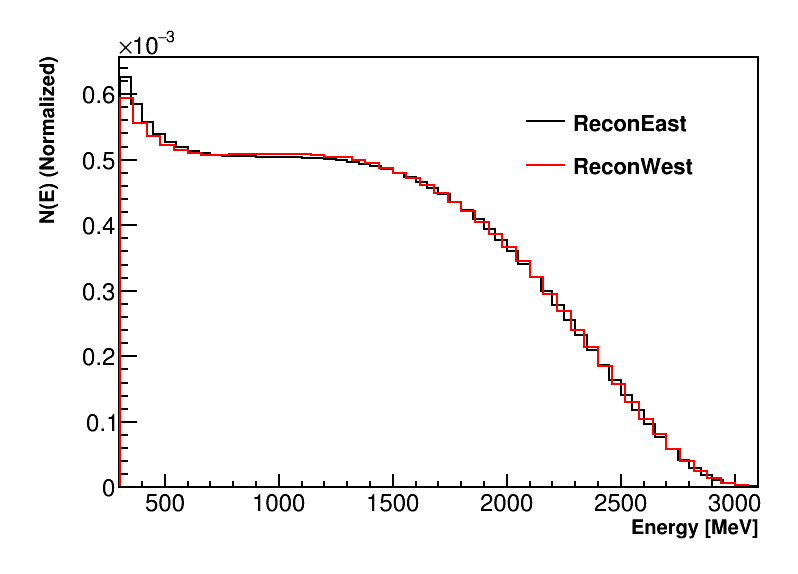
\includegraphics[width=\textwidth]{ReconEastvWest_N}
        \caption{}
    \end{subfigure}% %you need this % here to add spacing between subfigures

    \begin{subfigure}[t]{0.45\textwidth}
        \centering
        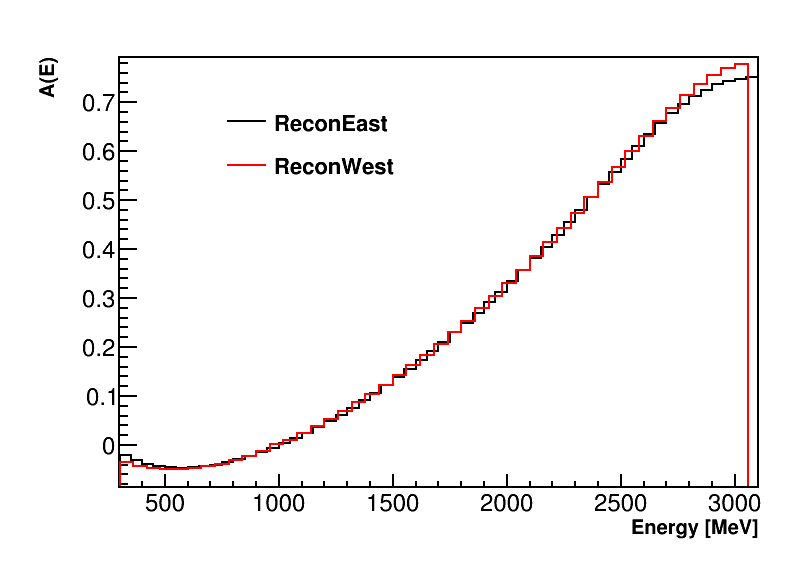
\includegraphics[width=\textwidth]{ReconEastvWest_A}
        \caption{}
    \end{subfigure}
    \hspace{1mm}
    \begin{subfigure}[t]{0.45\textwidth}
        \centering
        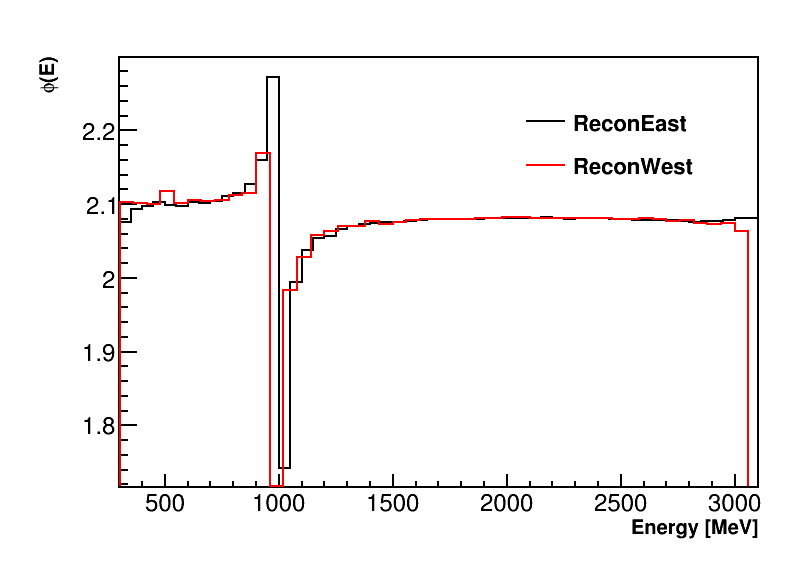
\includegraphics[width=\textwidth]{ReconEastvWest_Phi}
        \caption{}
    \end{subfigure}
\caption[]{Caption}
\label{fig:}
\end{figure}




\begin{figure}[]
\centering
    \begin{subfigure}[t]{0.45\textwidth}
        \centering
        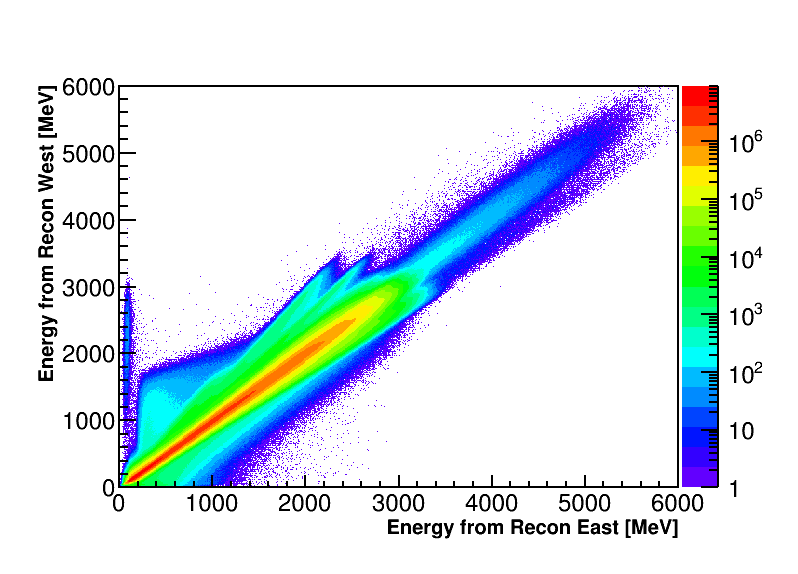
\includegraphics[width=\textwidth]{ReconEastvWest_Energies}
        \caption{}
    \end{subfigure}
    \hspace{1mm}
    \begin{subfigure}[t]{0.45\textwidth}
        \centering
        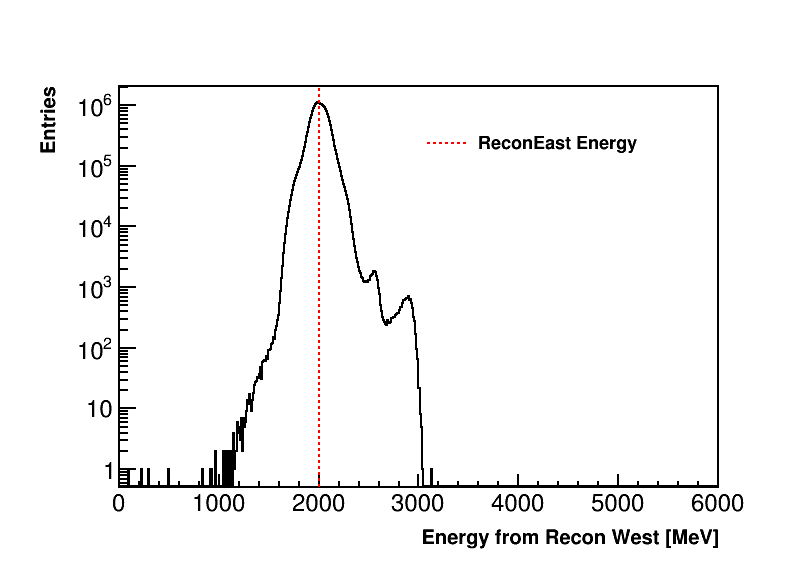
\includegraphics[width=\textwidth]{ReconEastvWest_Projection}
        \caption{}
    \end{subfigure}
\caption[]{Caption}
\label{fig:}
\end{figure}












- bring up datasets, etc. 

- don't do pileup, the effect should be a lot smaller than the energy threshold changes between analyses after pileup subtraction, it would be a major effort to somehow put in different pileup cases, etc.

